\begin{frame}
\frametitle{Charged Particle Tracking Reconstruction}

\begin{figure}[tbp]
\centering
%\includegraphics[width=0.3\linewidth]{PU140-RPhi.png}
%\includegraphics[width=0.3\textwidth]{tmp-RecoTimeLUMI_25_BX_25ns.png}
%\includegraphics[width=0.29\linewidth]{effandfake1_01.png}

%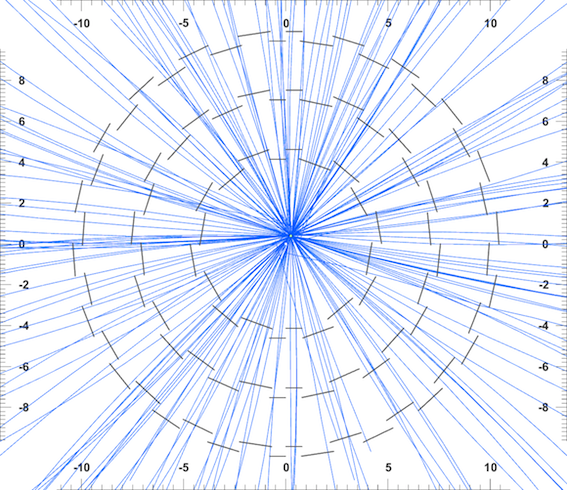
\includegraphics[width=0.32\linewidth]{images/PU50ns_run2_RPhi.png}
%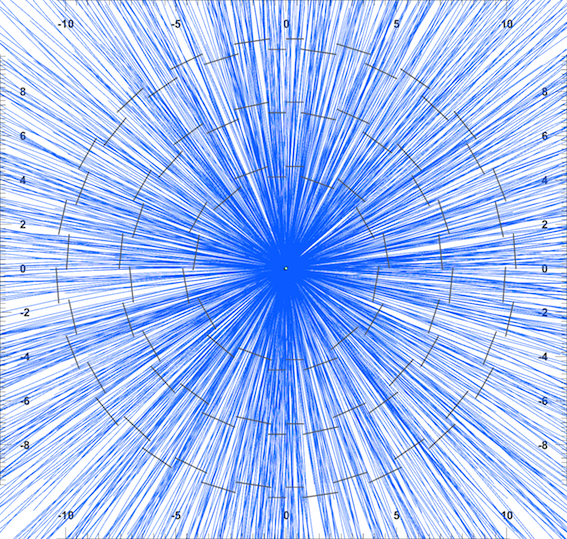
\includegraphics[width=0.3\linewidth]{images/PU140_2023_RPhi.png}
%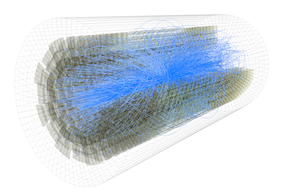
\includegraphics[width=0.3\linewidth]{images/PU140-3D.png}

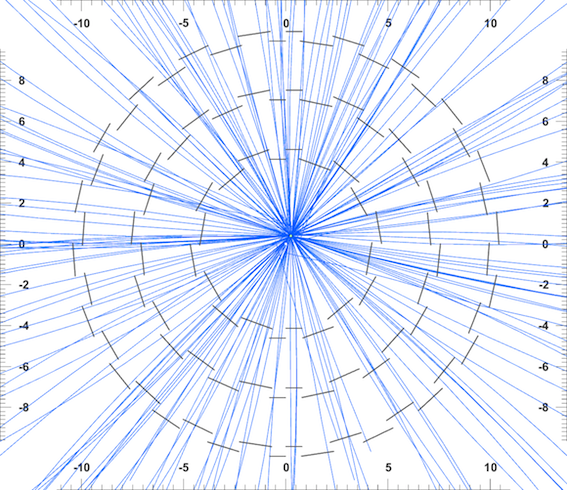
\includegraphics[width=0.5\linewidth]{images/PU50ns_run2_RPhi.png}
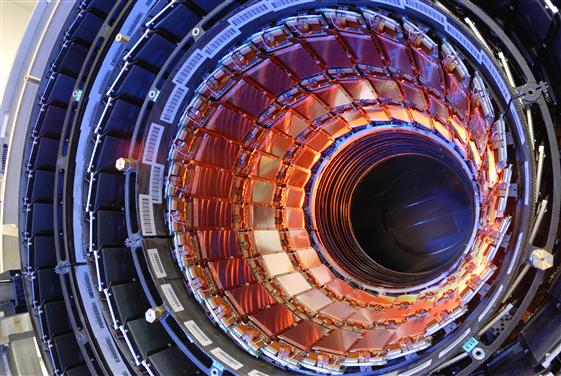
\includegraphics[width=0.5\linewidth]{images/0610026_01-A5-at-72-dpi.jpg}

%\caption{Display of charged particles in transverse plane to beams (r-phi) for
%PU=25 (2013) - left, and PU=140 (2023) - center, and 3D view of
%PU=140 collision - right.}
%\label{fig:PU140-All}
\end{figure}

%\small{Example Text}

\end{frame}


